\chapter{\textbf{Virtualization design advisor}}

\label{Virtualization design advisor}


In \cite{Soror:2008:AVM:1376616.1376711}, it is considered a typical scenario of resource consolidation, in which several DMBS instances, each one of them running in a separate VM, share a common pool of physical resources. The mentioned paper addresses the problem of optimizing the performance of these instances by controlling the configurations of the VMs in which they run. These configurations determine how these resources will be allocated to each DMBS instance. It's also considered that the physical resources belong to one server, in which all the VMs run. The scenario is illustrated in ~\ref{fig:scenario}.


\begin{figure}[ht]
\centering
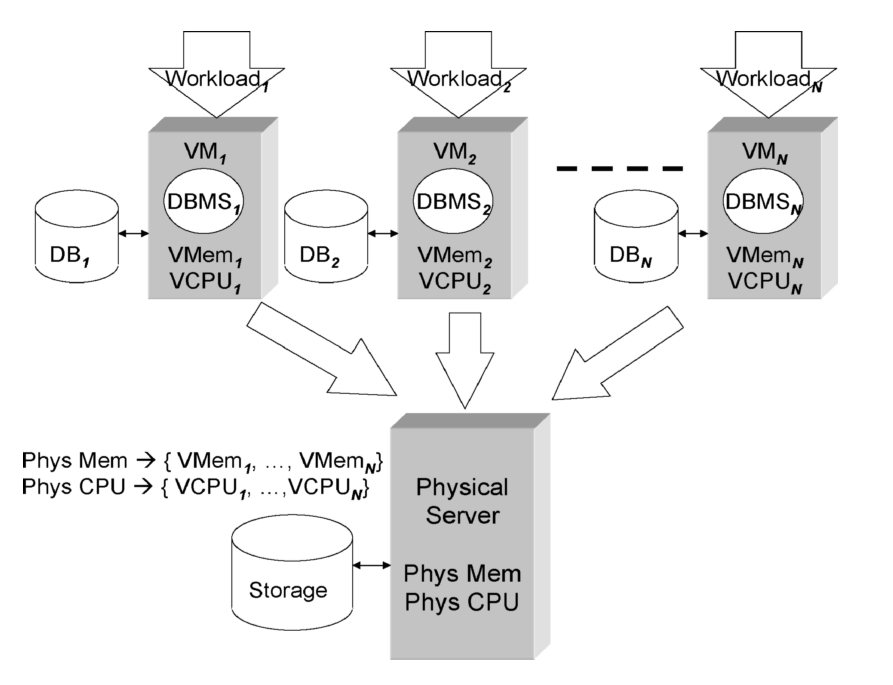
\includegraphics[width=0.8\textwidth]{dbms_consolidation.png}
\caption{Resource Consolidation scenario}
\label{fig:scenario}
\end{figure} 

\section{Problem definition}

In order to model this problem, the author assumes that there are  $M$ types of resources , such as CPU capacity, memory, or I/O bandwidth. The notation used to represent the share of resources allocated to a VM running a workload $W_{i}$ is $R_{i} = [r_{i1},...r_{iM}], 0 \leq r_{ij} \leq 1$. This workload represents the statements processed by the different DMBS instances at the same amount of time. 

Each workload has a cost, which depends on the resource share allocated to the VM in which it runs. It is used $Cost(W_{i},R_{i})$ to represent the cost of running the workload $W_{i}$ under resource allocation $R_{i}$. Considering that there are $N$ workloads, the goal is to choose $r_{ij}, 1 \leq i \leq N, 1 \leq j \leq M$ such that 
\[
  \sum_{i=1}^{N} Cost(W_{i},R_{i})
\]
is minimized.

This problem is generalized to satisfy Quality of Service (QoS) requirements.On of these requirements is to specify the maximum increase in cost that is allowed for a workload under the recommended resource allocation. It was defined a \textit{cost degradation} as
\[
 Degradation(W_{i},R_{i}) = \frac{Cost(W_{i},R_{i})}{Cost(W_{i},[1,...,1])}
\]
, where $[1,...,1]$ represents the resource allocation in which all the available resources are allocated to $W_{i}$. It can be specified a \textit{degradation limit} $L_{i} ( L_{i} \geq 1 )$, such that 
\[
 Degradation(W_{i}, R_{i}) \leq L_{i}
\]
for all $i$. This limit is set per workload, so it does not need information about other workloads that it will be sharing the physical server with.

The other QoS requirement introduced is the ability to specify relative priorities among the different workloads. A \textit{benefit gain factor} $G_{i} (G_{i} \geq 1)$ can be used to indicate how important is to improve the performance of $W_{i}$. Each unit of improvement is considered to worth $G_{i}$ cost units. When this parameter is applied to the problem, it may cause a workload to get more resources than its fair share. In order to incorporate it to our problem, the cost equation is modified to minimize the following
\[
  \sum_{i=1}^{N} G_{i} * Cost(W_{i},R_{i})
\]


\section{Architecture}

The process of  determining the allocation of resources to each VM is not immediate, nor static. The proposed advisor follows a sequence of steps. Initially, it makes resource allocations based on the workload descriptions and performance goals, which is performed offline, i.e., the VMs are not running yet. Then two following steps are performed online. First, it adjusts its recommendations based on workload costs to correct for any cost estimation erros made during the initial phase. Second, it uses continuing monitoring information to dynamically detect changes in the workloads. This last step is important because a workload cannot be considered static, its resource needs may change during execution. This approach prevents the advisor from allocating resources to DBMS instances that will obtain little benefit from them.

Since the advisor has a considerable number of sub-processes, it makes sense to organize it in modules. An overview of this advisor in a modular way is given in ~\ref{fig:architecture}. This paper intends to give a brief explanation of each module.


\begin{figure}[ht]
\centering
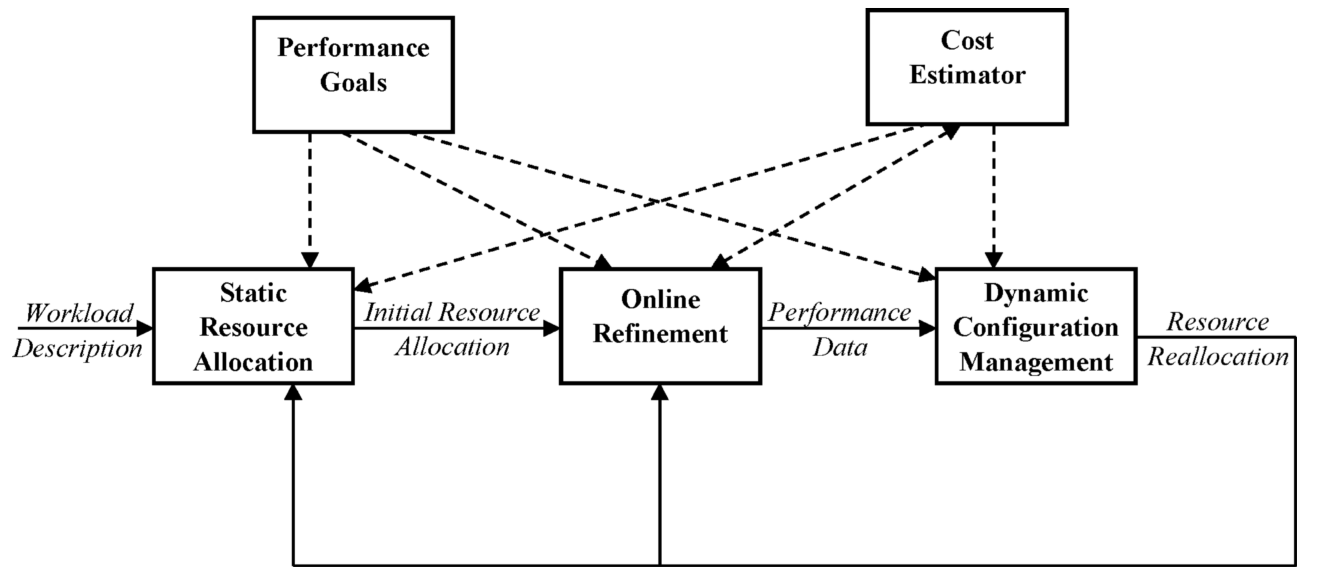
\includegraphics[width=0.8\textwidth]{architecture.png}
\caption{Advisor overview}
\label{fig:architecture}
\end{figure} 

\subsection{Cost estimator}

Given a workload $W_{i}$, the cost estimator will estimate $Cost(W_{i},R_{i})$. The strategy used to implement this module is to leverage the cost models built into database systems for query optimization. The query optimizer cost model can be described as $Cost_{DB}(W_{i},P_{i},D_{i})$, where $W_{i}$ is a SQL workload, $P_{i} = [p_{i1},..,p_{iL}]$ is a vector of parameters that are used to list both the available computing resources and DBMS configuration parameters relevant to the cost model, and $D_{i}$ is  the database instance. 

The author identifies two problems in using only query optimizer cost models. The first problem is the difficulty of comparing cost estimates produced by different DMBSes. They may have different cost models. Even if they share the same notion of cost, they normalize costs differently. This problem is addressed partially by the advisor. Although it only considers that the DBMSes have the same notion of cost, it proposes a renormalization step, in order to make $Cost_{DB}(W_{i},P_{i},D_{i})$ from different DBMSes comparable. For our purpose this step is not considered for implementation, since the support of multiple DBMSes is out of scope of this paper.

The second problem is that the query optimizer cost estimates depends on $P_{i}$, while the virtualization design advisor is given a candidate resource allocation $R_{i}$. The mapping of these two parameters is done through a calibration step. This step determines a set of DBMS cost model configuration parameters according to the different possible candidate resource allocations. It is supposed to be performed per DMBS on the physical machine before running the virtualization design advisor. Once the appropriate configuration parameters $P_{i}$ are determined for every possible $R_{i}$, the DBMS cost model is used to generate $Cost_{DB}$.

The calibration step is performed on  \textit{descritive parameters}, which are used to characterize the execution environment. The approach to the \textit{prescritive parameters}, which control the configuration of the DBMS itself, is to leave it for user definition. For instance, the ~\ref{table:descritive}  show some descritive parameters used in PostgreSQL, while ~\ref{table:prescritive}  show the prescritive ones. 


\begin{table}[ht]
    \centering
    \begin{tabular}{ | l | p{5cm} |}
    \hline
    Parameter & Description  \\ \hline
    \textbf{random\_page\_cost} & Cost of non-sequential page I/O \\ \hline
    \textbf{cpu\_tuple\_cost} & CPU cost of processing one tuple \\ \hline
    \textbf{effective\_page\_size} & size of file system's page size  \\
    \hline
    \end{tabular}
    \caption{Descritive parameters}
    \label{table:descritive}
\end{table}


\begin{table}[ht]
    \centering
    \begin{tabular}{ | l | p{5cm} |}
    \hline
      Parameter & Description  \\ \hline
    \textbf{shared\_buffers} & shared bufferpool size \\ \hline
    \textbf{work\_mem} & amount of memory used by each sort and hashing operator. \\
    \hline
    \end{tabular}
    \caption{Prescritive parameters}
    \label{table:prescritive}
\end{table}

The calibration follows the basic methodology for each parameter $p_{ij} \in P_{i}$:

\begin{itemize}
 \item (1) Define a calibration query $Q$ and a calibration database $D$, such that $Cost_{DB}(Q,P_{i},D)$ is independent for all descritive parameters in $P_{i}$, except for $p_{ij}$; \\
  \item (2) Choose a resource allocation $R_{i}$, instantiate $D$, and run $Q$ under that resource allocation, and measure the execution time $T_{Q}$; \\
  \item (3) This step refers to the renormalization of the $Cost_{DB}$ provided by the DBMS. As mentioned earlier in this section, we are not going into the details of this step; \\
  \item (4) Repeat the two preceding steps for a variety of $R_{i}$, associating with each parameter $p_{ij}$ that describes that resource. For instance, query optimizer parameters that describe CPU, I/O and memory are independent of each other and can be calibrated independently; \\
  \item (5) Perform regression analysis on the set of $(R_{i},p_{ik})$ value pairs to determine a calibration function $Cal_{ij}$ that maps resource allocations to $p_{ik}$ values. \\
\end{itemize}

During the described methodology, calibration queries should be carefully chosen. They need to be dependent only on the parameter that is being calibrated. If it is not possible to isolate one parameter, a system of $k$ equations is solved to determine the values for the $k$ parameters.


\section{Online refinement}

The initial allocation is based on the calibrated query optimizer cost model, as described earlier. This enables the advisor to make recommendations based on an informed cost model. However, this model may have inaccuracies that lead to sub-optimal recommendations. The  \textit{online refinement} is based on the observation the actual times of different workloads in the different virtual machines. It uses these observations to refine resource allocation recommendations. Then the advisor is rerun with the new cost models, so  we can obtain an improved resource allocation for different workloads. These optimizations are performed until the allocations stabilize. It's important to notice that the goal of the \textit{online refinement} is not deal with dynamic changes in the workload, which are dealt by another module, but to correct cost models. Thus, it's assumed that the workload is not going to change during this process. 


